\documentclass[11pt]{article}
\usepackage{setspace}
\setstretch{1}
\usepackage{amsmath,amssymb, amsthm}
\usepackage{graphicx}
\usepackage{bm}
\usepackage[hang, flushmargin]{footmisc}
\usepackage[colorlinks=true]{hyperref}
\usepackage[nameinlink]{cleveref}
\usepackage{footnotebackref}
\usepackage{url}
\usepackage{listings}
\usepackage[most]{tcolorbox}
\usepackage{inconsolata}
\usepackage[papersize={8.5in,11in}, margin=1in]{geometry}
\usepackage{float}
\usepackage{caption}
\usepackage{esint}
\usepackage{url}
\usepackage{enumitem}
\usepackage{subfig}
\usepackage{wasysym}
\newcommand{\ilc}{\texttt}
\usepackage{etoolbox}
\usepackage{algorithm}
\usepackage{changepage}
% \usepackage{algorithmic}
\usepackage[noend]{algpseudocode}
\usepackage{tikz}
\usetikzlibrary{matrix,positioning,arrows.meta,arrows}
\patchcmd{\thebibliography}{\section*{\refname}}{}{}{}
% \PassOptionsToPackage{hyphens}{url}\usepackage{hyperref}

\providecommand{\myceil}[1]{\left \lceil #1 \right \rceil }
\providecommand{\myfloor}[1]{\left \lfloor #1 \right \rfloor }


\begin{document}



\title{\textbf{CSDS 455: Homework 9}}

\author{Shaochen (Henry) ZHONG, \ilc{sxz517}}
\date{Due and submitted on 09/23/2020 \\ Fall 2020, Dr. Connamacher}
\maketitle

\section*{Problem 1}

\begin{proof}
Suppose we have $k$ edge-disjoint $a \to b$ paths in $G$, this suggest there are at least $k$ entirely distinct ways of getting from vertex $a$ to $b$. So intuitively, we need to cut out all of these paths to ensure $a$ to be disconnected from $b$. And it is known that to cut off a path, at least 1 edge needs to be removed, thus for a graph with $k$ edge-disjoint $a \to b$ paths, we need to remove $k$ edges to make $a$ to be disconnected from $b$.

Note when selecting an edge to remove from an edge-disjoint path, such edge must be an common edge of all paths from $a \to b$ which share edge(s) with this particular edge disjoint path.
\end{proof}

\section*{Problem 2}

\textit{I consulted \url{https://math.stackexchange.com/questions/3113602/} for this problem.}\newline

\begin{proof}

\leavevmode\newline


    \begin{adjustwidth}{1cm}{}

    \begin{proof}
    \textbf{Menger's Theorem: For a connected, finite undirected graph $G$. The minimum vertex cut for $u, v \in V(G)$ is equal to the maximum number of vertex-disjoint paths from $u$ to $v$}.\newline

    Say we have $k$ vertex-disjoint paths from $u$ to $v$. We will need to remove a vertex to break a path (similar to \textit{Problem 1}, we will need to remove the common vertex of all paths from $u$ to $v$ where these path has a shared vertex with the path we removing vertex from), so we must remove $k$ vertices to disconnect $u$ to $v$.

    \textbf{By promoting this proof to all vertex pairs, this means any $k$-connected graph will have k (internally) vertex-disjoint paths from any vertex pair in G.}


    \end{proof}

    \end{adjustwidth}

With the lemma proven, we may arbitrarily select $k$ desired vertices and find a cycle $C$ of $G$ which has $j$ common vertices with the $k$ desired vertex set (we call this set $D_k$), say $v_1, v_2, ..., v_j$. If $j = k$, then the statment is automatically proven. \newline

If $j < k$ but $|C| \geq k$, by the lemma and knowing that $G$ is a $k$-connected graph, we know that there must be $k$ vertex-disjoint paths from $C$ to $v_k$, where $v_k$ $\in D_k$ and $\not \in C$. We also know that these $k$ vertex-disjoint paths from $C$ to $v_k$ can end on $k$ different vertices on $C$.

Thus, we may find two adjacent vertices on $C$ (denotes them $v_i$ and $v_{i+1}$) and replace the edge between them with a path\footnote{This path must exist as there will be at least $k$ distinct vertices connecting $v_{i}$ or $v_{i+1}$ to $v_k$, so we can always connect $v_i$ to one of the vertex, reach $v_k$ via a path, and get back to $v_{i+1}$ from another vertex via another path. Notices we use two intermidiate vertices here, so the graph must be at least 2-connected} of $v_{i} \to v_k \to v_{i+1}$. Since there are $k$ paths between $C$ to any vertex in $D_k$, we may do replace-edge-with-a-path manuver entil all $k$ vertices in $D_k$ is included in the cycle.

If $j < k$ but $|C| = $k$-1$, there must be $k-1$ vertex-disjoint paths from $C$ to $v_k$, each ending on a different vertex on $C$. We know that $|C|$ must be $2$ as otherwise $C$ will not be a cycle, so we may always find two adjacent vertices $v_i$ and $v_{i+1}$ on $C$. Replace the edge between them with the path $v_{i} \to v_k \to v_{i+1}$, now we have included the only leftover desired vertex $v_k$ into the cycle.\newline

With $\geq k$ and $k-1$ both being true, and known that $k=2$ is trivially true\footnote{Due to any two vertices in a 2-connected graph will have 2 vertex-disjoint paths between them. So by identifying the two desired the vertices and connecting the two vertex-disjoint paths between them, we will automatically have a cycle containing them.}, we have proven the statement by induction.





\end{proof}

\section*{Problem 3}

\textit{I intensively discussed with Jiaqi Yu and Yuhui Zhang on this problem.}\newline

\noindent\textbf{$\Longrightarrow$ To prove by contrapositive, W.T.S. that if $G − \{x, y\}$ is not 2-connected, then $G/xy$ is not 3-connected.}

\begin{proof}
For $G - \{x, y\}$ to be not 2-connected, there must be $\kappa(G - \{x, y\}) < 2$. So either $\kappa(G - \{x, y\}) = 0$ where $G$ is already disconnected, then adding a point $v_{xy}$ will not make $G/xy$ become 3-connected as we can simply remove this $v_{xy}$ then we will have our $G - \{x, y\}$ with $\kappa(G - \{x, y\}) = 0$. In this case we have at most $\kappa(G/xy) = 1$, so $G/xy$ can't be 3-connected.

In case of $\kappa(G - \{x, y\}) = 1$, $\kappa(G/xy)$ is at most $2$. Because regardless what the $v_{xy}$ will be in $G/xy$, we can simply remove it, which will give us the 1-connectivity $G - \{x, y\}$ graph back, then we shall remove that 1 cut-off vertex in $G - \{x, y\}$ which will disconnect $G/xy$. Since we have at most $\kappa(G/xy) = 2$, $G/xy$ can't be 3-connected.\newline

Since the contrapositive is fulfilled, we have proven the forwards direction.

\end{proof}


\noindent\textbf{$\Longleftarrow$ To prove by contrapositive, W.T.S. that if $G/xy$ is not 3-connected, then $G − \{x, y\}$ is not 2-connected.}

\begin{proof}

Same as above, a not 3-connected $G/xy$ implies $\kappa(G/xy)$ is at most $2$. Also known that $G$ is 3-connected, which implies at least $\kappa(G) = 3$. Combine them together, we know that vertices $x, y$ must be both removed to disconnect $G$.\newline

We know this because if none of $x, y$ need to be removed to have a disconnected $G$ where $\kappa(G) = 3$, then $x, y$ and also $v_{xy}$ are not influential to the connectivity of their graphs, so we won't have a $\kappa(G/xy) \leq 2$ as the same 3 vertices also need to be removed in $G/xy$ to make $G/xy$ disconnect, a contradiction.

If one of $x, y$ but not both needs to be removed to to disconnect $G$ where $\kappa(G) = 3$. W.L.O.G. say $y$ is the one needs to be removed, then there must be two other vertices (say $A, B$) need to be removed to disconnect $G$. Which implies for vertices $u, v$ (where $u$ and $v$ are from different components of the the disconnected $G$), path $u \to x \to v$ must internally shares vertex(ices) with path $u \to A \to v$, $u \to B \to v$, or path $u \to y \to v$. Then in $G/xy$ we still need to break these 3 internally-vertex-disjoint paths to disconnect $G/xy$, which yields $\kappa(G/xy) = 3$, also a contraction to the setup.\newline

So only if vertices $x, y$ must be both removed to disconnect $G$, we shall then have a $G/xy$ with $\kappa(G/xy) \leq 2$ as now we can just removed the contracted $v_{xy}$ and have a $\kappa(G/xy) = 2$. However, in $G - \{x, y\}$, vertices $x$ and $y$ are already removed; this means $\kappa(G - \{x, y\}) = 1$ and $G - \{x, y\}$ is not 2-connected. This fulfills the contrapositive and proven the backwards direction.

\end{proof}
 % on one of the vertex-disjoint paths between the two disconnected component of $G$, thus by doing an edge contraction on $x, y$ to $v_{xy}$, we have decreased

% The to-be-prove statement is ``Let $G$ be a 3-connected graph. Prove that $G/xy$ is 3-connected if and only if $G − \{x, y\}$ is 2-connected.'' This suggests for a 3-connected $G$, if we have a 3-connected $G/xy$, we should be able to have a 2-connected $G − \{x, y\}$.\newline
%
% It seems I can find the below $G$ as a counterexample for this statement. It seems as long as the connectivity of $G$ is depended on vertices $x, y$, $G − \{x, y\}$ can have a uncontrollable connectivity. I don't know if it is due to my interpretation of the question instruction.
%
%
% \begin{figure}[H]
%     \centering
%     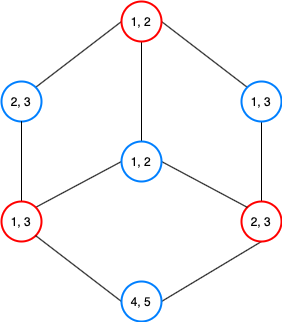
\includegraphics[width=1\linewidth]{{fig/fig_p3.png}}
%     \label{fig:3}
% \end{figure}





% \section{References}
%
% \nocite{*}
% \raggedright
% \bibliography{references.bib}
% \bibliographystyle{plain}


\end{document}